%%%%%%%%%%%%%%%%%%%%%%%%%%%%%%%%%%%%%%%%%%%%%%%%%%%%%%%%%%%%%%%%%%%%%%
% Lớp 11 | Đường thẳng, mặt phẳng. Quan hệ song song trong | Điểm, đường thẳng và mặt phẳng
% Dạng 1H4?1-2: Hình biểu diễn của một hình không gian
% Số câu: 9  (sinh tự động bởi tach_cau.py; từ nay thầy sửa trực tiếp file này)
%%%%%%%%%%%%%%%%%%%%%%%%%%%%%%%%%%%%%%%%%%%%%%%%%%%%%%%%%%%%%%%%%%%%%%

%%%%%%%%%%%%%%%% TRẮC NGHIỆM 4 PHƯƠNG ÁN %%%%%%%%%%%%%%%%

% nguồn: Ok_Toan11_TracNghiem_Lan2
\begin{ex}%[1H4N1-2]%[ma:b4dde02a]
	Trong các hình vẽ sau hình nào có thể là hình biểu diễn  của một hình tứ diện?
	\begin{center}
		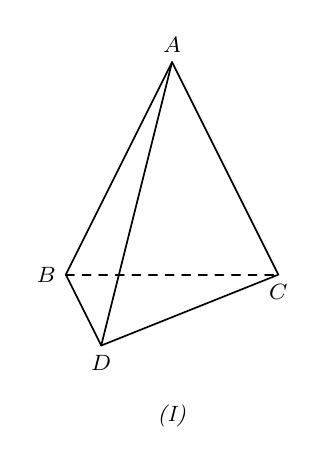
\begin{tikzpicture}[line join=round,line cap=round,line width=.6pt,font=\footnotesize,scale=0.9]
				\coordinate[label=left:$B$] (B) at (0,0); 
				\coordinate[label=below:$C$] (C) at  (3,0);
				\coordinate[label=below:$D$] (D)  at (0.5,-1);
				\coordinate[label=above:$A$] (A) at (1.5,3); 
				 \draw (A)--(B)--(D)--(C)--cycle;
				\draw  (A)--(D);
				 \draw[dashed] (B)--(C);
				\node at (1.5,-2)  {\textit{(I)}};
			\end{tikzpicture}
		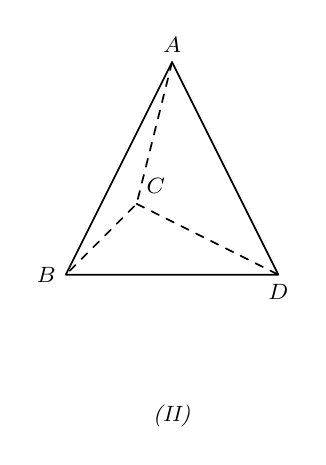
\begin{tikzpicture}[line join=round,line cap=round,line width=.6pt,font=\footnotesize,scale=0.9]
				\coordinate[label=left:$B$]  (B) at (0,0);
				\coordinate[label=below:$D$] (D)  at (3,0);
				\coordinate[label=above right:$C$] (C) at (1,1); 
				\coordinate[label=above:$A$]  (A) at (1.5,3);
				\draw  (A)--(B)--(D)--cycle;
				\draw[dashed]  (C)--(D)
					 (A)--(C)--(B);
				 \node at (1.5,-2) {\textit{(II)}};
			\end{tikzpicture}
		\begin{tikzpicture}[line join=round,line cap=round,line width=.6pt,font=\footnotesize,scale=0.9]
				\coordinate[label=left:$B$] (B) at (0,0); 
				\coordinate[label=below:$C$] (C) at  (3,0);
				\coordinate[label=below right:$D$]  (D) at (4,0);
				\coordinate[label=above:$A$] (A) at (1,3); 
				\draw (A)--(B)--(D)--cycle; 
				 \draw (A)--(C);
				\node at  (1.5,-2) {\textit{(III)}};
			\end{tikzpicture}
		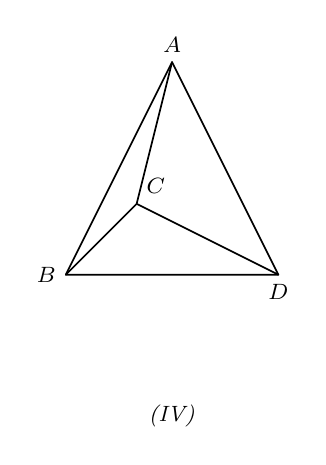
\begin{tikzpicture}[line join=round,line cap=round,line width=.6pt,font=\footnotesize,scale=0.9]
				\coordinate[label=left:$B$] (B)  at (0,0);
				\coordinate[label=below:$D$] (D) at  (3,0);
				\coordinate[label=above right:$C$]  (C) at (1,1);
				\coordinate[label=above:$A$] (A)  at (1.5,3);
				\draw  (A)--(B)--(D)--cycle;
				 \draw (A)--(C)--(D)
					(B)--(C); 
				 \node at (1.5,-2) {\textit{(IV)}};
			\end{tikzpicture}
	\end{center}
	 \choice
		{\True $(I),\,(II),\,(IV)$} 
		 {$(I),\,(II),\,(III),\,(IV)$}
		{$  (I)$}
		{$  (I),\,(II),\,(III)$}
	\loigiai{ 
	Hình $ (III)$ không phải là hình biểu  diễn của một hình tứ diện.}
\end{ex}

% nguồn: Ok_Toan11_TracNghiem_Lan2
\begin{ex}%[1H4N1-2]%[ma:436bc9a5]
	Trong các hình vẽ sau đâu  là hình biểu diễn của hình tứ diện?
	 \def\dotEX{}
	\choice 
		{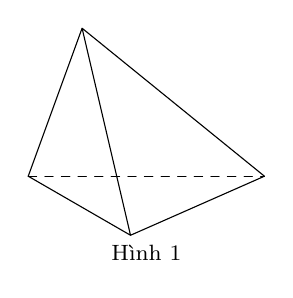
\begin{tikzpicture}[scale=1,font=\footnotesize,line join=round,line cap=round,>=stealth]
		\path (0,0) coordinate  (B)
			(3,0) coordinate (D) 
			(-30:1.5) coordinate  (C)
			(70:2)  coordinate (A);
		 \draw (A)--(B)--(C)--(D)--cycle (C)--(A);
		\draw[dashed] (B)--(D); 
		\path (current bounding box.south) node[below]{Hình  $1$};
	\end{tikzpicture}
		} 
		{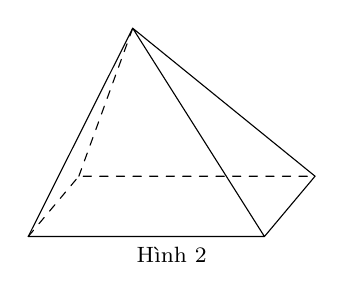
\begin{tikzpicture}[scale=1,font=\footnotesize,line join=round,line cap=round,>=stealth]
		\path (0,0)  coordinate (A)+(-130:1) coordinate (D)
			 (3,0) coordinate (B)+(-130:1) coordinate (C)
			 (70:2) coordinate (S);
		\draw  (S)--(D)--(C)--(B)--cycle (S)--(C);
		 \draw[dashed] (S)--(A)
			 (D)--(A)--(B);
		 \path (current bounding box.south) node[below]{Hình $2$};
	\end{tikzpicture}
		} 
		{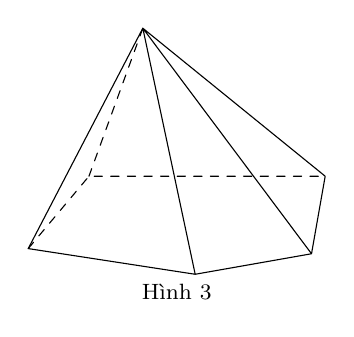
\begin{tikzpicture}[scale=1,font=\footnotesize,line join=round,line cap=round,>=stealth]
		\path (0,0) coordinate  (A)++(-130:1.2) coordinate (E)
			(3,0) coordinate (B)++(-100:1) coordinate (C)++(-170:1.5)  coordinate (D)
			 (70:2) coordinate (S);
		 \draw (S)--(B)--(C)--(D)--(E)--cycle (C)--(S)--(D);
		\draw[dashed]  (S)--(A)
			 (E)--(A)--(B);
		\path (current  bounding box.south) node[below]{Hình $3$};
	\end{tikzpicture}
		} 
		{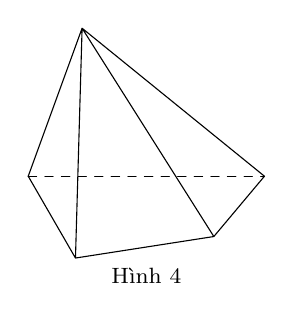
\begin{tikzpicture}[scale=1,font=\footnotesize,line join=round,line cap=round,>=stealth]
		\path (0,0) coordinate  (A)+(-60:1.2) coordinate (D)
			(3,0) coordinate (B)+(-130:1)  coordinate (C)
			 (70:2) coordinate (S);
		\draw (S)--(A)--(D)--(C)--(B)--cycle  (D)--(S)--(C);
		\draw[dashed]  (A)--(B);
		\path  (current bounding box.south) node[below]{Hình $4$};
	\end{tikzpicture}
		} 
	 \loigiai{
		Ta có Hình $1$ là hình biểu diễn của một tứ diện. 
	 }
\end{ex}

% nguồn: Ok_Toan11_TracNghiem_Lan2
\begin{ex}%[1H4N1-2]%[ma:fea5c281]
	Trong các hình vẽ sau hình nào là hình biểu diễn của một hình  tứ diện?
	\begin{center}
		\begin{tabular}{cccc}
			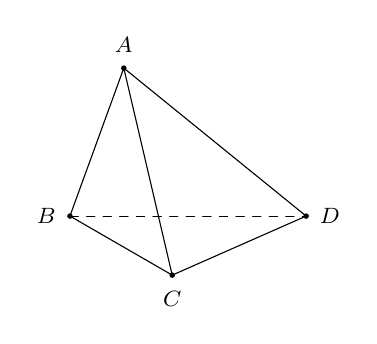
\begin{tikzpicture}[scale=1,font=\footnotesize,line join=round,line cap=round,>=stealth]
					\path (0,0)  coordinate (B)
						(3,0)  coordinate (D)
						(-30:1.5) coordinate (C) 
						(70:2) coordinate  (A);
					\draw (A)--(B)--(C)--(D)--cycle (C)--(A); 
					\draw[dashed] (B)--(D); 
					\foreach \x/\g in  {A/90,B/180,C/-90,D/0}{
						\fill (\x) circle (1pt)+(\g:0.3) node{$\x$}; 
					} 
				\end{tikzpicture}
			 &
			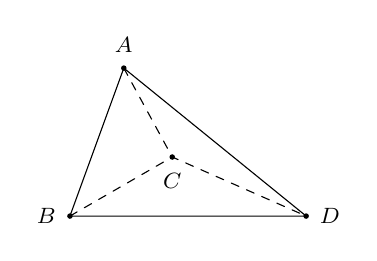
\begin{tikzpicture}[scale=1,font=\footnotesize,line join=round,line cap=round,>=stealth]
					\path (0,0) coordinate  (B)
						(3,0)  coordinate (D)
						 (30:1.5) coordinate (C)
						(70:2)  coordinate (A);
					 \draw (A)--(B)--(D)--cycle;
					\draw[dashed] (B)--(C)--(D) 
						(A)--(C); 
					 \foreach \x/\g in {A/90,B/180,C/-90,D/0}{
						\fill  (\x) circle (1pt)+(\g:0.3) node{$\x$};
					} 
				\end{tikzpicture}
			& 
			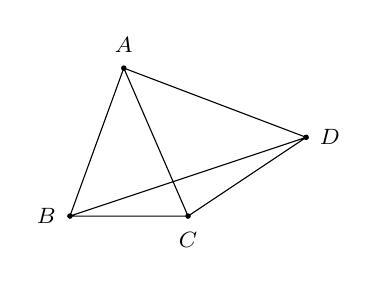
\begin{tikzpicture}[scale=1,font=\footnotesize,line join=round,line cap=round,>=stealth]
					\path (0,0)  coordinate (B)
						(3,1) coordinate (D) 
						(0:1.5) coordinate (C) 
						 (70:2) coordinate (A);
					\draw (A)--(B)--(C)--(D)--cycle (A)--(C) 
						 (B)--(D);
					\foreach \x/\g in  {A/90,B/180,C/-90,D/0}{
						\fill (\x) circle (1pt)+(\g:0.3)  node{$\x$};
					 }
				\end{tikzpicture}
			 &
			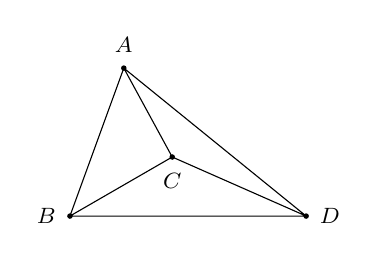
\begin{tikzpicture}[scale=1,font=\footnotesize,line join=round,line cap=round,>=stealth]
					\path  (0,0) coordinate (B)
						 (3,0) coordinate (D)
						 (30:1.5) coordinate (C)
						(70:2) coordinate (A); 
					\draw  (A)--(B)--(D)--cycle (A)--(C)--(D)
						 (C)--(B);
					\foreach \x/\g in {A/90,B/180,C/-90,D/0}{ 
						\fill (\x) circle  (1pt)+(\g:0.3) node{$\x$};
					} 
				\end{tikzpicture}
			\\ 
			Hình $1$ & Hình $2$  & Hình $3$ & Hình $4$
		\end{tabular}
	\end{center}
	\choice 
		{\True Hình $1$, Hình $2$, Hình  $4$}
		{Hình $1$, Hình $2$,  Hình $3$, Hình $4$}
		 {Hình $1$}
		{Hình $1$,  Hình $2$, Hình $3$}
	\loigiai{ 
		Các Hình $1$, Hình $2$,  Hình $4$ biểu diễn một hình tứ diện.\\
		Hình $3$ không phải  là hình biểu diễn của một hình tứ diện vì điểm $AC$ và $BD$ là các nét liền, cắt nhau nên $ABCD$ là tứ giác.
	 }
\end{ex}

% nguồn: Ok_TracNghiemLop11_Lan1
\begin{ex}%[1H4N1-2]%[ma:48bfac3a]
	Cho hình chóp $S.ABCD$, gọi $O$ là giao điểm của $AC$ và $BD$. Lấy $M$, $N$ lần lượt thuộc các cạnh $SA$, $SC$. Đường thẳng nào  sau đây \textbf{không} thuộc mặt phẳng $(SAC)$.
	\begin{center}
		\begin{tikzpicture}[scale=0.7,font=\footnotesize,line join=round,line cap=round,>=stealth]
				\path 
					(0,0) coordinate  (A)
					 ++(-140:3) coordinate (B)
					++(0:5) coordinate  (C)
					 ($(A)+(C)-(B)$) coordinate (D)
					($(A)+(1,4)$)  coordinate (S)
					 ($(S)!0.5!(A)$) coordinate (M)
					($(S)!0.5!(C)$) coordinate (N) 
					($(A)!0.5!(C)$) coordinate  (O);
				\foreach \i in{B,C,D}{\draw (S)--(\i);}; 
				\draw (B)--(C)--(D); 
				\draw[dashed]  (S)--(A)--(B)--(D)--(A)--(C)
					 (M)--(N);
				 \foreach \i/\g in {A/-90,B/-90,C/-90,D/-60,S/90,M/30,N/30,O/-90}
				\fill[black] (\i)  circle (1pt)+(\g:5mm) node[scale=1]{$\i$};
			\end{tikzpicture}
	\end{center}
	\choice 
		 {$SA$}
		{$MN$} 
		 {$AC$}
		{\True  $BO$}
	 \loigiai{
		\begin{center}
			\begin{tikzpicture}[scale=0.7,font=\footnotesize,line join=round,line cap=round,>=stealth]
					 \path
						(0,0) coordinate  (A)
						++(-140:3) coordinate  (B)
						++(0:5)  coordinate (C)
						($(A)+(C)-(B)$) coordinate  (D)
						 ($(A)+(1,4)$) coordinate (S)
						($(S)!0.5!(A)$)  coordinate (M)
						($(S)!0.5!(C)$)  coordinate (N)
						 ($(A)!0.5!(C)$) coordinate (O);
					 \foreach \i in{B,C,D}{\draw (S)--(\i);};
					\draw  (B)--(C)--(D);
					\draw[dashed]  (S)--(A)--(B)--(D)--(A)--(C)
						 (M)--(N);
					\foreach  \i/\g in {A/-90,B/-90,C/-90,D/-60,S/90,M/30,N/30,O/-90}
					\fill[black] (\i) circle  (1pt)+(\g:5mm) node[scale=1]{$\i$};
				\end{tikzpicture}
		\end{center}
		Ta  có $S$, $A$, $C$, $M$, $N \in (SAC)$ nên $SA$, $SC$, $MN\subset (SAC)$.\\
		Mặt khác $\heva{&B \not\in (SAC)\\&O\in (SAC)\\} \Rightarrow BO \not\subset  (SAC)$.
	 }
\end{ex}

% nguồn: Ok_TracNghiemLop11_Lan1
\begin{ex}%[1H4N1-2]%[ma:ddac4ea7]
	Một hình chóp có đáy là ngũ giác có số mặt và số  cạnh là
	 \choice
		{$6$ mặt,  $5$ cạnh}
		{\True  $6$ mặt, $10$ cạnh}
		{$5$ mặt, $10$ cạnh} 
		{$5$ mặt, $5$ cạnh} 
	 \loigiai{\immini{
		Hình chóp ngũ giác có $5$ mặt bên và $1$ mặt đáy,  $5$ cạnh bên và $5$ cạnh đáy.}{
		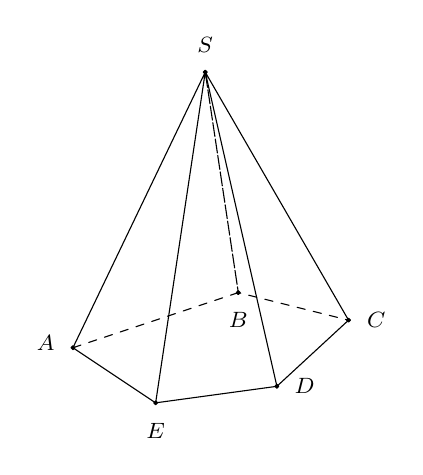
\begin{tikzpicture}[line join=round,line cap=round,>=stealth,scale=0.7,font=\footnotesize]
				\tikzset{every node/.style={outer  sep=-0.5mm}}
				\foreach \x/\y/\n in {0/0/A,3.7/-0.7/D,3/1/B,5/0.5/C,2.4/5/S,1.5/-1/E} \coordinate (\n)  at (\x,\y);
				\draw (S)--(A)--(E)--(D)--(C)--(S)--(D)--(E)--(S); 
				\draw[dashed] (A)--(B)--(S)--(B)--(C); 
				\foreach  \t/\g in {A/170,B/-90,C/0,D/0,S/90,E/-90}{
					\draw[fill] (\t) circle (1pt) node[shift={(\g:10pt)}]{$ \t $};} 
			\end{tikzpicture}
		 }
	} 
\end{ex}

% nguồn: Ok_TracNghiemLop11_Lan1
\begin{ex}%[1H4N1-2]%[ma:50b0ccb0]
	Trong  các hình sau
	\begin{center}
		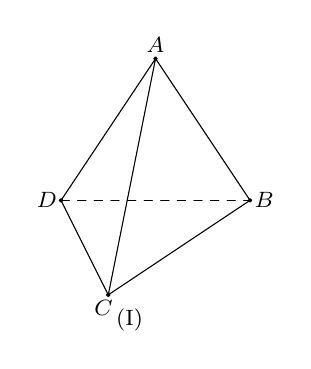
\begin{tikzpicture}[scale=0.6,font=\footnotesize,line join=round,line cap=round,>=stealth]
				 \def\h{4}
				 \path
					 (0,0) coordinate (D)
					(1,-2) coordinate  (C)
					(4,0)  coordinate (B)
					 (2,3) coordinate (A)
					(C)+(-50:0.7)  node{(I)};
				\draw 
					(D)--(C)--(B) 
					(A)--(B) 
					(A)--(C) 
					(A)--(D); 
				\draw[dashed] (D)--(B); 
				\foreach \p/\g in  {A/90,B/0,C/-110,D/180}
				\draw[fill] (\p) circle (1pt)+(\g:0.3) node{$\p$}; 
			\end{tikzpicture}
		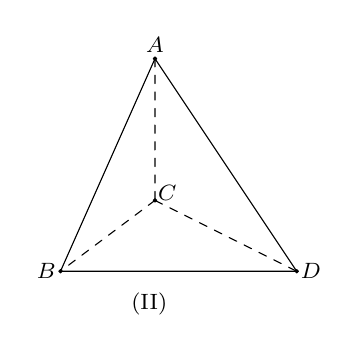
\begin{tikzpicture}[scale=0.6,font=\footnotesize,line join=round,line cap=round,>=stealth]
				\def\h{4} 
				 \path
					 (0,0) coordinate (B)
					(2,1.5)  coordinate (C)
					 (5,0) coordinate (D)
					(2,4.5) coordinate  (A)
					(B)+(-20:2) node{(II)}; 
				 \draw
					 (A)--(B)--(D)--cycle;
				\draw[dashed] 
					(C)--(B) 
					(A)--(C) 
					 (C)--(D);
				\foreach \p/\g in  {A/90,B/180,C/30,D/0}
				\draw[fill] (\p) circle (1pt)+(\g:0.3) node{$\p$}; 
			\end{tikzpicture}
		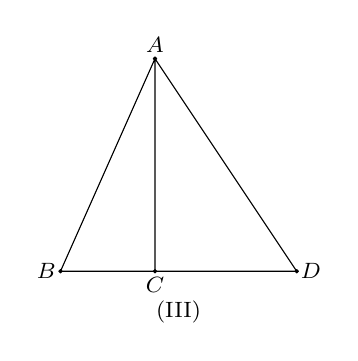
\begin{tikzpicture}[scale=0.6,font=\footnotesize,line join=round,line cap=round,>=stealth]
				 \def\h{4}
				 \path
					 (0,0) coordinate (B)
					 (2,0) coordinate (C)
					(5,0) coordinate (D) 
					(2,4.5) coordinate (A) 
					(C)+(-60:1)  node{(III)};
				 \draw
					(A)--(B)--(D)--cycle 
					(A)--(C); 
				\foreach \p/\g in {A/90,B/180,C/-90,D/0} 
				\draw[fill] (\p)  circle (1pt)+(\g:0.3) node{$\p$};
			\end{tikzpicture}
		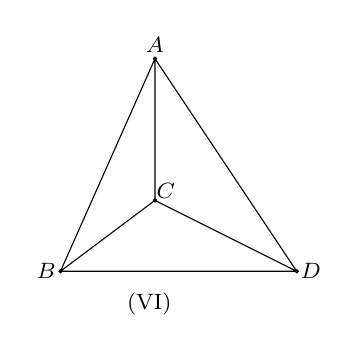
\begin{tikzpicture}[scale=0.6,font=\footnotesize,line join=round,line cap=round,>=stealth]
				 \def\h{4}
				\path 
					(0,0) coordinate (B) 
					(2,1.5) coordinate (C) 
					(5,0) coordinate  (D)
					(2,4.5) coordinate  (A)
					(B)+(-20:2)  node{(VI)};
				\draw 
					(A)--(B)--(D)--cycle 
					 (C)--(B)
					(A)--(C) 
					(C)--(D); 
				\foreach  \p/\g in {A/90,B/180,C/40,D/0}
				\draw[fill] (\p) circle  (1pt)+(\g:0.3) node{$\p$};
			\end{tikzpicture}
	\end{center}
	Hình nào có thể là hình biểu diễn của một hình  tứ diện?
	\choice 
		 {(I)}
		 {(I), (II)}
		{(I), (II),  (IV)}
		 {\True (I), (II), (III), (IV)}
	\loigiai{ Tất cả các hình trên đều có thể là biểu diễn của một tứ diện. 
	 }
\end{ex}

% nguồn: Ok_TracNghiemLop11_Lan1
\begin{ex}%[1H4N1-2]%[ma:6f522940]
	Cho hình chóp $S.ABCD$ có đáy $ABCD$ là hình thang, đáy lớn $AB$ gấp đôi đáy nhỏ $CD$, $E$ là trung điểm của đoạn $AB$. Hình  vẽ nào sau đây đúng quy tắc?
	 \choice
		{\begin{tikzpicture}[line join = round,line cap = round,font=\footnotesize,>=stealth,scale=1]
		\coordinate (B) at (-1,1); 
		\coordinate (A) at (3,2); 
		\coordinate (C) at  (0,0);
		\coordinate  (D) at (2,0);
		\coordinate (S)  at (-1,4);
		\coordinate (E)  at ($(A)!0.5!(B)$);
		\draw  (B)--(C)--(D)--(A)
			 (C)--(S)--(B)
			 (A)--(S)--(D);
		 \draw[dashed](B)--(A);
		\foreach  \i/\g in {A/0,B/180,C/-90,D/-90,S/90,E/90}{\draw[fill](\i) circle (1pt)
			($(\i)+(\g:3mm)$)  node[scale=1]{$\i$};}
	\end{tikzpicture}
		} 
		{\begin{tikzpicture}[line join = round,line cap = round,font=\footnotesize,>=stealth,scale=1]
		\coordinate  (B) at (-1,1);
		 \coordinate (A) at (3,1);
		\coordinate (C) at  (0,0);
		\coordinate (D) at  (2,0);
		\coordinate (S) at (-1,4); 
		\coordinate (E)  at ($(A)!0.5!(B)$);
		 \draw (A)--(B)--(C)--(D)--(A)
			 (C)--(S)--(B)
			 (A)--(S)--(D);
		\foreach \i/\g in {A/0,B/180,C/-90,D/-90,S/90,E/90}{\draw[fill](\i) circle (1pt) 
			 ($(\i)+(\g:3mm)$) node[scale=1]{$\i$};}
	\end{tikzpicture}
		 }
		{\True \begin{tikzpicture}[line join = round,line cap = round,font=\footnotesize,>=stealth,scale=1]
		\coordinate  (B) at (-1,1);
		 \coordinate (A) at (3,1);
		 \coordinate (C) at (0,0);
		\coordinate (D)  at (2,0);
		 \coordinate (S) at (-1,4);
		 \coordinate (E) at ($(A)!0.5!(B)$);
		\draw (B)--(C)--(D)--(A) 
			 (C)--(S)--(B)
			(A)--(S)--(D); 
		 \draw[dashed](B)--(A);
		\foreach  \i/\g in {A/0,B/180,C/-90,D/-90,S/90,E/-90}{\draw[fill](\i) circle (1pt)
			($(\i)+(\g:3mm)$)  node[scale=1]{$\i$};}
	\end{tikzpicture}
		 }
		{\begin{tikzpicture}[line join = round,line cap = round,font=\footnotesize,>=stealth,scale=1]
		\coordinate  (B) at (-1,1);
		\coordinate (A) at (3,1); 
		 \coordinate (C) at (0,0);
		\coordinate (D) at  (2,0);
		\coordinate  (S) at (-1,4);
		\coordinate (E) at  ($(B)!0.7!(A)$);
		\draw (B)--(C)--(D)--(A) 
			 (C)--(S)--(B)
			(A)--(S)--(D); 
		\draw[dashed](B)--(A); 
		\foreach \i/\g in {A/0,B/180,C/-90,D/-90,S/90,E/90}{\draw[fill](\i)  circle (1pt)
			($(\i)+(\g:3mm)$) node[scale=1]{$\i$};} 
	\end{tikzpicture}
		 }
	 \loigiai{
		 Hình vẽ đúng qui tắc là hình vẽ sau:
		\begin{center}
			\begin{tikzpicture}[line join = round,line cap = round,font=\footnotesize,>=stealth,scale=1]
					 \coordinate (B) at (-1,1);
					\coordinate (A) at (3,1); 
					\coordinate (C) at  (0,0);
					\coordinate (D) at (2,0); 
					\coordinate (S) at  (-1,4);
					\coordinate  (E) at ($(A)!0.5!(B)$);
					\draw (B)--(C)--(D)--(A) 
						 (C)--(S)--(B)
						 (A)--(S)--(D);
					 \draw[dashed](B)--(A);
					\foreach \i/\g in {A/0,B/180,C/-90,D/-90,S/90,E/-90}{\draw[fill](\i) circle  (1pt)
						 ($(\i)+(\g:3mm)$) node[scale=1]{$\i$};}
				\end{tikzpicture}
		\end{center}
	} 
\end{ex}

% nguồn: Ok_TracNghiemLop11_Lan1
\begin{ex}%[1H4H1-2]%[ma:3a3c953f]
	Hình  chóp lục giác có bao nhiêu mặt bên?
	 \choice
		{$5$} 
		{\True $6$} 
		 {$3$}
		 {$4$}
	 \loigiai{
		Hình chóp lục giác có $6$  mặt bên.
	} 
\end{ex}

% nguồn: Ok_TracNghiemLop11_Lan1
\begin{ex}%[1H4Y1-2]%[ma:5a5e2501]
	Hình tứ diện có số cạnh  là
	\choice 
		{$3$} 
		 {\True $6$}
		 {$5$}
		 {$4$}
	\loigiai{ 
		\begin{center}
			\begin{tikzpicture}[scale=0.8,font=\footnotesize,line join=round,line cap=round,>=stealth]
					\coordinate [label= left:  $D$](D) at (0,0);
					\coordinate [label= below:  $B$](B) at (2,-2);
					\coordinate [label=  right: $C$](C) at (6,0);
					\coordinate [label=  above: $A$](A) at ($(D)+(1,4)$);
					 \draw (A)--(D)--(B)--(C)--(A)--(B);
					\draw[dashed] (D)--(C); 
					\foreach  \i in {A,B,C,D} \draw[fill] (\i) circle (1.1pt);
				\end{tikzpicture}
		\end{center}
		Hình tứ diện có $6$ cạnh. 
	 }
\end{ex}
